\documentclass{article}

\usepackage{listings}
\usepackage{color}
\usepackage{graphicx}
\usepackage{float}
\usepackage{amsmath}
\usepackage{subfig}
\usepackage{cite}
\usepackage{url}

\begin{document}

\title{$\mu$Image Manipulator}

\author{Hamid Mirisaee,
\and Jander Nascimento, 
\and Raquel Oliveira}

\maketitle

\tableofcontents

\section{Filters}

	\subsection{Fundamental}

		By definition, a filter is a device or process which removes some unwanted features from an image (more precisely, from a signal).
		Low-pass and high-pass filters are regarded as  classic examples of filters in image processing field. Generally, filters are used to be convolved 
		(the convolution is described in the next part) with an image in order to produce a new, modified image. This new image, in turn, could
		be used for some other processing. The next subsection will introduce the convolution and its basics.
		
		\subsubsection{Convolution}

			Convolutions are used to perform many useful image processing tasks such as noise reduction and edge detection. Generally,
			convolution is a mathematical operation on two functions f and g to produce a modified version of one of the functions.
			Mainly, but not necessarily, the first function (signal) is the input and is bigger than the second one.
			The following formulas describe the discrete convolution formula in 1D and 2D space:

			\begin{equation}
			y[n] = f[n]*g[n] = \sum_{k=-\infty}^{+\infty} f[k]g[n-k]
			\end{equation}
			\begin{equation}
			y[m,n] = f[m,n]*g[m,n] = \sum_{i=-\infty}^{+\infty}\sum_{j=-\infty}^{+\infty}f[i,j]g[m-i,n-j]
			\end{equation}

			
			When dealing with finite-length signals, one cannot use the ordinary convolution formula (called linear convolution).
			In such cases, the circular convolution, which results in zeros outside of the range of the signal, is used. The mathematical formula of discrete 
			convolution could be seen in the following:
			\begin{equation}
			y[n] = f[n]*g[n] = \sum_{k=-K/2}^{+K/2} f[k]g[n-k]
			\end{equation}
			\begin{equation}
			y[m,n] = f[m,n]*g[m,n] = \sum_{i=-K/2}^{+K/2}\sum_{j=-T/2}^{+T/2}f[i,j]g[m-i,n-j]
			\end{equation}


			
			
			In image processing field, generally, the input image is the first function of the convolution, and the second 
			function is considered as the kernel or filter.
			In this context we use the terms kernel and filter interchangeably.
			There is a wide range of filters which are used to perform different tasks on a given image. The next subsection would go through some of these 
			filters which are used in the application in addition to a brief description for each of them.

		\subsection{Used filters}
		
		\subsubsection{Gaussian}

			The Gaussian kernel is a 2D convolution operator which is used to blur an image and remove noise. Mostly, applying a convolution using a Gaussian
			kernel is called Gaussian smoothing. Generally, the Gaussian kernel is centered at
			zero (pick at 0). The following describes the Gaussian formula in 2D space:
\begin{equation}
			G(x,y) = \frac{1}{2\pi\sigma^{2}}e^{-\frac{x^{2}+y^{2}}{2\sigma^{2}}}
\end{equation}
			
			Gaussian smoothing acts almost the same as the mean filter, which will be in the following part. The following figures illustrates a noisy image and its blurred copy using a 5 by 5 Gaussian kernel

	\begin{figure} [H]
		\centering
		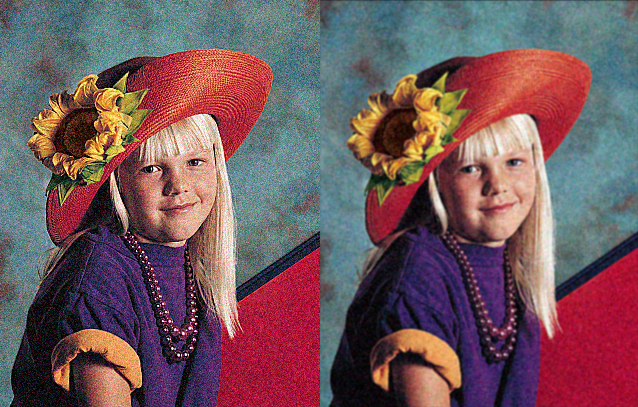
\includegraphics[scale=0.3]{images/noisy_removed}
		\caption{Left side: noisy image Right side: blurred image \label{crop_1}}
	\end{figure}


		\subsubsection{Mean}
			Mean filter is an easy to implement kernel which is used to reduce the noise in an image by reducing the amount of intensity variation between one
			pixel and the next. The idea of the mean filter is to replace the value of each pixel with the average of its neighbors including itself. In the figure \ref{mean} an example of mean filter is shown.
\begin{figure}[H]
\begin{center}
 \begin{tabular}{ | l | c | r | }
    \hline
    1/9 & 1/9 & 1/9 \\ \hline
    1/9 & 1/9 & 1/9 \\ \hline
    1/9 & 1/9 & 1/9 \\
    \hline
  \end{tabular}
\end{center}
\caption{3 by 3 example of mean filter \label{mean}}\end{figure}
		
		\subsubsection{Gradient}

			Applying gradient filter to an image is one of the edge detection approaches. Before explaining the gradient filter and its properties, we will see a
			short description of the edge detection concept. 
			
			Technically, an edge is a part of image where a considerable change is occurred in the brightness of the pixels.
			More informally, edges are the boundaries of
			the objects in an image. Detecting edges in an image is a non-avoidable issue in some image processing tasks such as intelligent resizing.
			
			Mathematically, gradient is the first derivation of the signal. In other words, it is a vector with a certain magnitude and direction. 
			The magnitude of the gradient provides information about strength
			of the edge, and the direction of the gradient is always perpendicular to the direction of the edge. Clearly, the gradient filter could be
			applied horizontally and vertically. The gradient vector is given below:
\begin{equation}
  \bigtriangledown f = \begin{pmatrix}
\frac{\partial f}{\partial x} = M_x\\ 
\frac{\partial f}{\partial y} = M_y
\end{pmatrix}
\end{equation}
\begin{equation}
magn(\bigtriangledown f) = \sqrt{M_x^{2}+M_y^{2}}\approx \left | M_x \right |+\left | M_y \right |
\end{equation}
\begin{equation}
dir(\bigtriangledown f) = \tan^{-1}(\frac{M_y}{M_x})
\end{equation}



			There are several filters based on the gradient concept. Sobel edge detector and Prewitt edge detector are two well-known filters in this regard.
			As it is mentioned previously, gradient approach is based on the first derivation of the input. Based on the properties of
			the first derivative, the edges of a given input could be seen near the picks in the first derivative curve. Accordingly, a threshold should be
			determined in order for the edges to be detected. However, since a thresholding is used, the edges might be too thick to be considered
			as an edge. As a result, we may need to apply a localization method (for instance, using Laplacian filter) to find zero
			crossing points and separate actual edges from other non-edge points. Figure \ref{pre}  illustrates the horizontal Prewitt operator. The vertical is the transpose of the horizontal filter. Also, Figure \ref{edge} illustrates an image with its edge-detected copy using Prewitt filters.


\begin{figure}[H]
\begin{center}
 \begin{tabular}{ | l | c | r | }
    \hline
    -1 & 0 & 1 \\ \hline
    -1 & 0 & 1 \\ \hline
    -1 & 0 & 1 \\
    \hline
  \end{tabular}
\end{center}
\caption{Horizontal Prewitt operator\label{pre}}\end{figure}
	\begin{figure} [H]
		\centering
		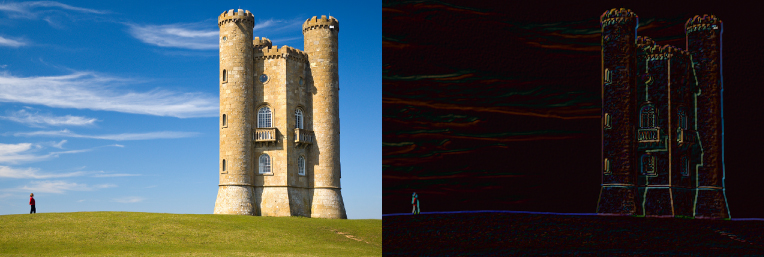
\includegraphics[scale=0.4]{images/edged}
		\caption{Left side: original image. Right side: edge-detected image based on Prewitt filters \label{edge}}
	\end{figure}

		
		\subsubsection{Laplacian}
			The Laplacian filter is computed based on the second derivative of the input. The following matrix is an approximation of a 3 by 3 Laplacian filter; however, a 5 by 5 filter is used in the developed application based on better results it produced for
most of the tested images.

\begin{figure}[H]
	\begin{center}
  \begin{tabular}{ | l | c | r | }
    \hline
    -1 & -1 & -1 \\ \hline
    -1 & 8 & -1 \\ \hline
    -1 & -1 & -1 \\
    \hline
  \end{tabular}
\end{center}
\caption{an example of a 3 by 3 Laplacian filter}\end{figure}



			 Since the Laplacian filter is based on the second derivative of the input, it is highly sensitive to noise. Consequently,
			it is generally applied after a noise reduction process. Alternatively, one can use LoG (Laplacian of Gaussian) since the convolution operation is
			associative. The following is the LoG formula in 2D space:

\begin{equation}
			LoG(x,y) = -\frac{1}{\pi\sigma^{4}}[1-\frac{x^{2}+y^{2}}{2\sigma^{2}}]e^{-\frac{x^{2}+y^{2}}{2\sigma^{2}}}
\end{equation}


\section{Color space}    
	A color space is a model by which the color are represented by a few numbers, typically three or four. Using primary colors, a vast variety of colors could be made. Two well-known models are RGB and CYMK.      

	\subsection{RGB}
		In RGB model, red, green and blue lights are added together to make a wide range of colors. This model is generally used in electronic systems such as CRTs and LCDs. In case of an 8-bit value for each color, more than 16 million different colors
		could be made using this model. The RGB model is considered as an additive model, which means the white color is a result of combination of all lights while black is a result of absence of all the lights.
	

	\subsection{CYMK}

		CMYK (Cyan, Magenta, Yellow, Key black) is another color model which is used in color printing. Unlike the RGB, CMYK is a subtractive; that is, white is is the natural color of the paper and black is a full mixture of all colors.
		As a result, to save money on ink, the dark colors and the black is produced using the black ink.

	\subsection{Gray scale conversion}

		In order to convert an image from an RGB colors to gray scale, we need to consider how far a pixel is from the black color. To achieve this goal, one can substitute all the colors of a pixel with the average of the three colors. Using this method, a pure black pixel would remain black, and a white pixel would still remain white. Other pixels, however, would have a gray view between black and white.

\section{Cropping}

	Cropping is a technique where the main purpose is to change or improve the visibility of a certain object in an image, 
	what is done by removing external frames. 
	The new target becomes the main object of the image generating a new image with the dimension of the target area.  

	\begin{figure}[H]
	\centering
	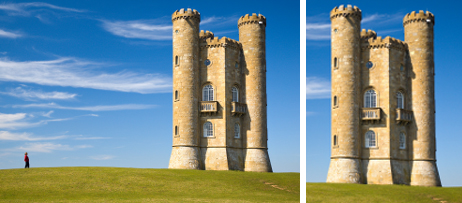
\includegraphics[scale=2]{images/crop}
	\caption{Left side: original image. Right side: cropped image}
	\label{fig:cropping}
	\end{figure}


\section{Fusion}

	The fusion operation is done by merging two images. The merging is based on the Equation \ref{eq:fusion}. 
	
	The $\alpha$ is a floating point value that represents the percentage of participation in the new image. 

	\begin{equation}
		f(pixel_{current},pixel_{to\ merge},\alpha)=(1-\alpha)*pixel_{current}+\alpha*pixel_{to\ merge}
		\label{eq:fusion}
	\end{equation}

\section{Resizing}

	Image resizing is defined as converting an image to a size in which may or may not respect the previous ratio size.
	When dealing with reducing the size of an image, it is quite simple to do it; however, when dealing with enlarging 
	the image, the process is a little bit more complex due to unknown pixels.

	Reducing the dimension of an image consists in removing as many lines and as many columns as necessary to reach target dimension. Obviously, this
	process may create some side-effects in the image, like Moiree pattern.

	When we stretch an image, we have few known pixels.

	There are many algorithms that helps us to guess those unknown pixels, for instance:

	\begin{itemize}
	  \item Nearest neighbor interpolation
	  \item Linear interpolation
	  \item Bilinear interpolation
	  \item Bi-cubic interpolation
	\end{itemize}

	The adopted algorithm is \textbf{Bilinear interpolation}  due to its speed and simplicity.
	
\subsection{From Linear to Bilinear interpolation}

	The Linear interpolation may be done horizontally or vertically, or even both. If a horizontal or vertical interpolation is done, we call it
	Linear interpolation. In case of applying both interpolations, its called Bilinear interpolation.	

	The pixel interpolation is done by calculating the mean of the known pixels around (vertical and horizontal axis) the unknown pixel. 

	\begin{figure} [H]
		\centering
		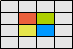
\includegraphics[scale=1]{images/bilinear_interpolation_1}
		\caption{original image \label{bilinear1}}
	\end{figure}

	In Figure \ref{bilinear1}, we can see the original image where all pixel are known pixels. Now what happens if we stretch this image 
	from a 2x2 to a 3x3 image?
	
	\begin{figure} [H]
		\centering
		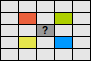
\includegraphics[scale=1]{images/bilinear_interpolation_2}
		\caption{image resized from 2x2 to 3x3 \label{bilinear2}}
	\end{figure}

	As we can see, after stretching the image to the desired dimension we create some unknown pixels. For those pixels, we can apply the linear interpolation. To guess the color intensity, the color of it's neighbor pixels are used (not by simply copying the neighbor).

	The example in the Figure \ref{bilinear2}, is not realistic for several reasons. First, in the most of the cases we must fill more than one gap in between known pixels. Second reason is that in real cases we consider the pixel in the horizontal and vertical direction, instead of diagonal axis. The third is that in the 
	previous example the distance between the unknown pixels and the known pixels were always the same, so a regular division would solve the problem. 
A more realistic example would be Figure \ref{bilinear3}.
	
	\begin{figure} [H]
		\centering
		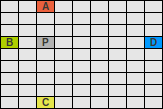
\includegraphics[scale=1]{images/bilinear_interpolation_3}
		\caption{more realistic image\label{bilinear3}}
	\end{figure}
	
	In this example, we can see that the interpolation cannot be only the mean of the pixels, since the unknown pixel 
	is closer to the pixels A and B. It is reasonable that this unknown pixel receives A and B colors more than the other ones.

	Consider \textit{distance(p1,p2)} a function that returns the distance between two pixels, 
	and \textit{color(p1)} a function that returns the color of the pixel \textit{p1} . First, we perform the Linear interpolation horizontally.
	\begin{equation}
	 f_h(p)=color(B)*\frac{distance(P,D)}{distance(B,D)}+color(D)*\frac{distance(B,P)}{distance(B,D)}  
	\end{equation}
	Secondly, we perform this operation in the vertical axis as well:
	\begin{equation}
	 f_v(p)=color(A)*\frac{distance(P,C)}{distance(A,C)}+color(C)*\frac{distance(A,P)}{distance(A,C)}
	\end{equation}

	Combining these two approaches, we have the bilinear interpolation.

	
\section{Histogram}

	\subsection{Color histogram}

		The histogram is an important tool when dealing with image analysis. It shows the color distribution of a certain image regarding to its 
		color \textit{spectrum}.
			
		The histogram is represented in a Cartesian, where \textit{x} axis is the 
		color \textit{spectrum} and \textit{y} represents the number of pixels.

		We may use two techniques
		to represent colorful images, either by summing all the colors into a single histogram, or create a different histogram for each color.
		

	\subsection{Normalization}
		
		The normalization, or histogram stretching, is a technique by which the color histogram is used to evaluate and possibly change
		the color intensity range. This enhances the detail level of some images that might appear too dark or too bright. This is done by spreading the pixels to use the entire color \textit{spectrum}.
		
		\begin{figure}[H]
		  \centering
		  \subfloat[Un-normalized]{\label{fig:nonnormalized}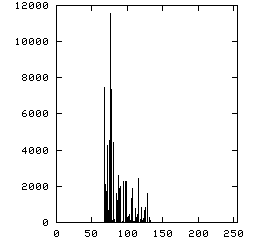
\includegraphics[width=0.3\textwidth]{images/histogram_1}}                
		  \subfloat[Normalized]{\label{fig:normalized}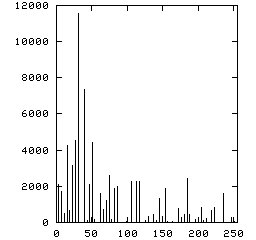
\includegraphics[width=0.3\textwidth]{images/histogram_2}}
		  \caption{Histogram normalization}
		  \label{fig:normalization}
		\end{figure}

		

		To normalize, the only variables we must know is the minimum and maximum color in the current histogram, 
		and minimum and maximum color in the enhanced histogram, or we may translate as a new position for the minimum and maximum colors. It is possible
		to write mathematically the Equation \ref{eq:normalization}. \nocite{*}


		\begin{equation}
			normalize(p)=new_{min}+\frac{new_{max}-new_{min}}{current_{max}-current_{min}}*(p-current_{min})
			\label{eq:normalization}
		\end{equation}
		

\section{Intelligent Resizing}

	One of the most important features in image manipulation softwares is the capability of resizing images. The classical resizing methods do not take into account the content of the image. In the crop method the user selects the most important part of the image and discard the other parts. The scale method distorts the content of the image. The Seam Carving method supports content-aware resizing by finding seams (least important paths) either to be removed or duplicated in the image (Figure \ref{intelligent1}).

	\begin{figure} [H]
		\centering
		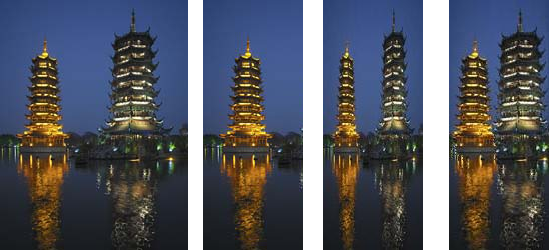
\includegraphics[scale=0.5]{images/intelligent3}
		\caption{Comparison between resizing methods. From left to right: the original image, resizing using crop, scaling and seam removal.\label{intelligent1}}
	\end{figure}

	\subsection{Seams}
	A seam is a connected path which begins in one extremity of the image and ends in the opposite extremity. A seam is a set of pixels which are selected horizontally or vertically. In order to perform a content-aware resize of the image, paths should be detected correctly. This is achieved by analyzing the energy of the image, which can be generate with algorithms like entropy, eye-gaze movement, visual saliency and gradient magnitude. In this software, the gradient magnitude is used based on good results it produced~\cite{ref:seamwiki}. This point is illustrated in Figure \ref{castle}.

	\begin{figure} [H]
		\centering
		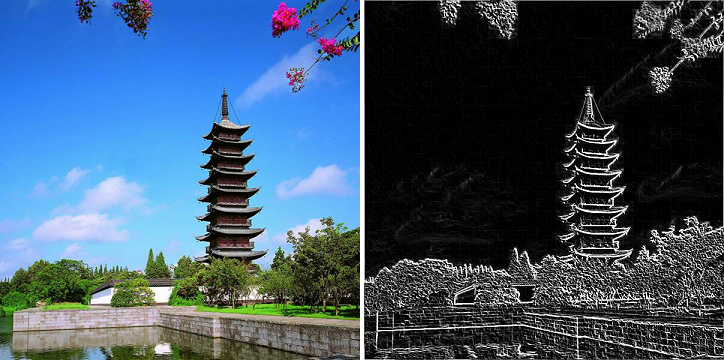
\includegraphics[scale=0.3]{images/intelligent2}
		\caption{The effect of gradient magnitude in a image\label{castle}}
	\end{figure}

	
	\subsection{Removing seams}
	Remove a seam is a four-step process. First, the gradient magnitude of the original image is made. Second,  we find the energy matrix using the Dijkstra's algorithms in order to compute the accumulative energy of each pixel. Third, we find the shortest path in the energy matrix. Afterwards, we remove this path from the original image and repeat the steps until the desired size is reached.

\bibliography{report}{}
\bibliographystyle{plain}

\end{document}

